% This file was created with matplot2tikz v0.5.4.
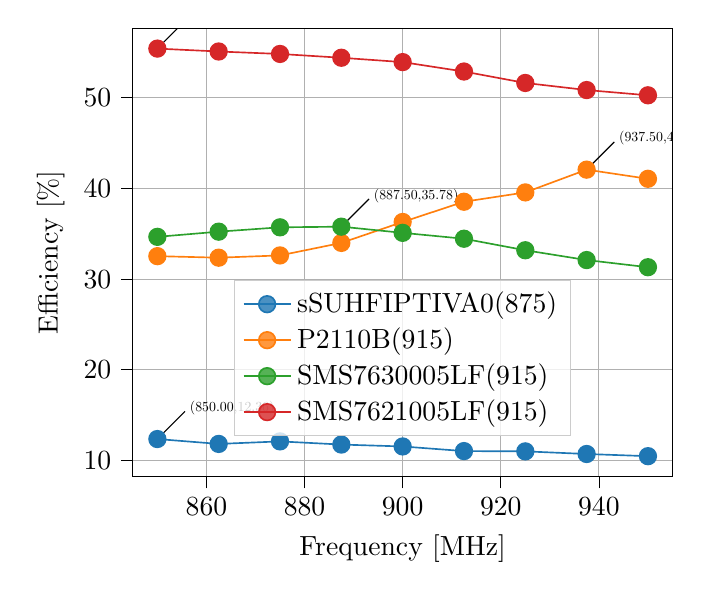
\begin{tikzpicture}

\definecolor{crimson2143940}{RGB}{214,39,40}
\definecolor{darkgray176}{RGB}{176,176,176}
\definecolor{darkorange25512714}{RGB}{255,127,14}
\definecolor{forestgreen4416044}{RGB}{44,160,44}
\definecolor{lightgray204}{RGB}{204,204,204}
\definecolor{steelblue31119180}{RGB}{31,119,180}

\begin{axis}[
legend cell align={left},
legend style={
  fill opacity=0.8,
  draw opacity=1,
  text opacity=1,
  at={(0.5,0.09)},
  anchor=south,
  draw=lightgray204
},
tick align=outside,
tick pos=left,
x grid style={darkgray176},
xlabel={Frequency [MHz]},
xmajorgrids,
xmin=845, xmax=955,
xtick style={color=black},
y grid style={darkgray176},
ylabel={Efficiency [\%]},
ymajorgrids,
ymin=8.2225, ymax=57.6675,
ytick style={color=black}
]
\addplot [semithick, steelblue31119180, mark=*, mark size=3, mark options={solid}]
table {%
850 12.36
862.5 11.82
875 12.1
887.5 11.75
900 11.54
912.5 11.03
925 11
937.5 10.71
950 10.47
};
\addlegendentry{sSUHFIPTIVA0(875)}
\addplot [semithick, darkorange25512714, mark=*, mark size=3, mark options={solid}]
table {%
850 32.53
862.5 32.36
875 32.61
887.5 33.99
900 36.3
912.5 38.53
925 39.56
937.5 42.07
950 41.06
};
\addlegendentry{P2110B(915)}
\addplot [semithick, forestgreen4416044, mark=*, mark size=3, mark options={solid}]
table {%
850 34.66
862.5 35.23
875 35.71
887.5 35.78
900 35.1
912.5 34.45
925 33.18
937.5 32.1
950 31.31
};
\addlegendentry{SMS7630005LF(915)}
\addplot [semithick, crimson2143940, mark=*, mark size=3, mark options={solid}]
table {%
850 55.42
862.5 55.1
875 54.83
887.5 54.41
900 53.93
912.5 52.89
925 51.63
937.5 50.85
950 50.27
};
\addlegendentry{SMS7621005LF(915)}
\draw[->,draw=black] (axis cs:850,12.36) ++(10pt,10pt) -- (axis cs:850,12.36);
\draw (axis cs:850,12.36) ++(10pt,10pt) node[
  scale=0.5,
  anchor=base west,
  text=black,
  rotate=0.0
]{(850.00,12.36)};
\draw[->,draw=black] (axis cs:937.5,42.07) ++(10pt,10pt) -- (axis cs:937.5,42.07);
\draw (axis cs:937.5,42.07) ++(10pt,10pt) node[
  scale=0.5,
  anchor=base west,
  text=black,
  rotate=0.0
]{(937.50,42.07)};
\draw[->,draw=black] (axis cs:887.5,35.78) ++(10pt,10pt) -- (axis cs:887.5,35.78);
\draw (axis cs:887.5,35.78) ++(10pt,10pt) node[
  scale=0.5,
  anchor=base west,
  text=black,
  rotate=0.0
]{(887.50,35.78)};
\draw[->,draw=black] (axis cs:850,55.42) ++(10pt,10pt) -- (axis cs:850,55.42);
\draw (axis cs:850,55.42) ++(10pt,10pt) node[
  scale=0.5,
  anchor=base west,
  text=black,
  rotate=0.0
]{(850.00,55.42)};
\end{axis}

\end{tikzpicture}
